% !TeX root = ../tfm.tex
%! TEX root = ../tfm.tex

En este capítulo expondremos las tareas realizadas para obtener una base de datos propia para el posterior entrenamiento del sistema, así como la descripción de la misma y de los estudios previos de las tramas obtenidas que nos ayudarán en el capítulo siguiente a la definición del modelo y parámetros del algoritmo.

Como ya hemos presentado anteriormente en la sección \ref{sec:req:bases_datos}, nos encontramos ante la falta de una base de datos para entrenar el modelo del producto final. Al tratarse de un modelo experimental es necesario conseguir un conjunto de datos lo más parecido posible a los capturados por la plataforma física utilizada. A su vez es necesario validar la capacidad de esta plataforma para servir al propósito de este trabajo. Así, con esta doble tarea de generar una bases de datos y confirmar que la plataforma cubre nuestras necesidades funcionales realizamos el primer desarrollo propio del trabajo.

\section{Captura de datos: AccelCapture}\label{sub:imp:accelcapture}

\textit{AccelCapture} es el nombre del sistema de captura de tramas de la aceleración capturada por el sensor situado en un reloj inteligente con sistema operativo \textit{WearOS}. Consta de dos componentes: una unidad de adquisición de datos, el propio reloj, y una segunda unidad de almacenamiento situada en la nube. Tal y como puede apreciarse en el diagrama de clases de la figura \ref{fig:accelcaptureClasesUml} la aplicación en si misma se compone de tres bloques funcionales.

\figura[0.47]{accelcaptureClassUML}{fig:accelcaptureClasesUml}{Diagrama de clases de AccelCapture}

\paragraph{MainWearActivity}
El punto de entrada de la aplicación. Genera la interfaz de usuario y permite introducir el nombre el usuario a la vez que verificar el estado del servicio de captura de datos e iniciar o parar su ejecución.

\paragraph{SensorsReader}
Un servicio que al ser creado se registra para recibir eventos y lecturas del sensor de aceleración triaxial del reloj. Posee una cola circular donde almacena los últimos 5 segundos de muestras (si por ejemplo la velocidad de lectura del sensor es de $1/50$, el buffer posserá $50 * 5 = 250$ muestras).
Este servicio realiza el análisis de la aceleración para detectar movimiento según el algoritmo definido en la figura \ref{fig:capturaFlow}. Tras cada muestra el algoritmo evalúa la variación de la aceleración según la fórmula: 

\[
  \Delta A_{i}=\left\{
    \begin{array}{lcl}
      |A_i - g|       & si & i = 0 \\
      |A_i - A_{i-1}| & si & i > 0 \\
    \end{array}
    \right.
\]

Donde $g$ corresponde a la aceleración de la gravedad terrestre o $9,8m/s^2$. Este valor $\Delta A_i$ se utiliza para realizar la detección de actividad mediante dos mecanismos:

\figura[0.55]{capturaFlujo}{fig:capturaFlow}{Flujo de trabajo de la aplicación AccelCapture}

\begin{enumerate}
  \item \textbf{Movimiento repentino} Se activa si la muestra leida es mayor de $2g$.
  \item \textbf{Movimiento prolongado} Activado cuando la aceleración promedio del contenido del buffer es superior a $0,3m/s^2$
\end{enumerate}

La cota de detección de movimiento repentino se calcula a partir de los resultados obtenidos por \citeA{Bourke2006} para la medición de la cintura por ser la que menor aceleración registra. La diferencia entre la aceleración de pico y de valle usada por bourke es de $\Delta A = (2,74 - 0,60)g = 2,14g$ redondeando a la baja a $2g$ para garantizar la detección de todos los eventos de este tipo. Finalmente, la cota del detector de actividad prolongada, fijada en $0,3m/s^2$, se mide de forma experimental resultado de promediar el vector para realizar el movimiento de leer la hora en el reloj (figura\ref{fig:accelMirarReloj}) y volver a la posición de reposo durante la ventana de 5 segundos que usa la aplicación. En caso de activarse alguno de estos mecanismos, el servicio considera que ha detectado una actividad y manda el contenido del buffer al servidor para ser guardado. 

\figura{MirarRelojAccel}{fig:accelMirarReloj}{$|A|$ y $\Delta A$ de resultantes de mirar el reloj}

El código de las funciones lambda puede consultarse el el apéndice \ref{app:code:accelcapturelambda} mientras que el de la aplicación AccelCapture está disponible para descarga en \url{https://github.com/aberaza/accelCapture}.

\subsection{Interfaz de Usuario}

La interfaz de usuario de la aplicación permite gestionar y observar el estado del servicio de captura así como definir el identificador de usuario al que pertenece la sesión. Como puede observarse en las capturas de pantalla de la figura\ref{fig:accelcapture:UI} se muestra en la parte inferior de la pantalla un boton con información del estado actual del servicio. El botón al ser pulsado alterna entre los estados \textit{activado} y \textit{desactivado}. En la parte superior de la pantalla se muestra la información del identificador de usuario o \textit{nombre} al que se asociarán todas las sesiones registradas. Este identificador puede modificarse desde el mismo reloj. Una vez activado el servicio de captura, puede esconderse interfaz y volver al modo reloj ya que el servicio sigue trabajando de fondo. 
\begin{figure}[htb!]
  \centering
  \begin{subfigure}[b]{0.4\textwidth}
      \centering
      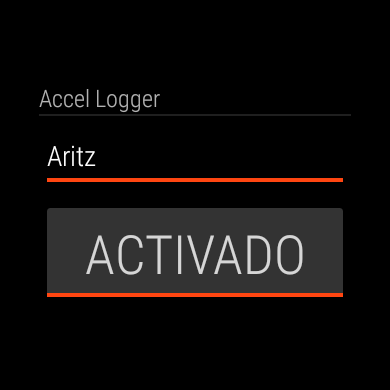
\includegraphics[width=\textwidth]{accelCaptureAct.png}
      \caption{AccelCapture Activado}
      \label{fig:accelCapture:UI1}
  \end{subfigure}
  \hfill
  \begin{subfigure}[b]{0.4\textwidth}
      \centering
      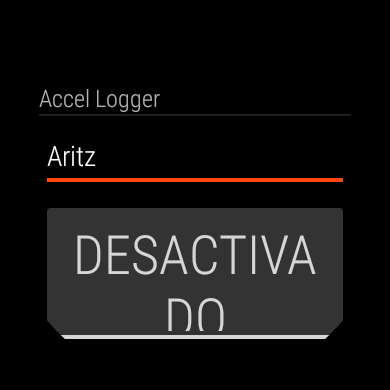
\includegraphics[width=\linewidth]{accelCaptureDes.png}
      \caption{AccelCapture Desactivado}
      \label{fig:accelCapture:UI2}
  \end{subfigure}
  \caption{\label{fig:accelcapture:UI} Interfaz de usuario de AccelCapture}
\end{figure}

\subsection{Almacenamiento de datos}

\tabla[0.65\linewidth]{tab:accelcapture:api}{API del servidor AccelCapture}{llll}{
  Método  & URL         & Carga         & Función lambda    \\ \hline
  POST    & /saveAccel  & AccelSession  & doGuardarAccel()  \\
}\todo{poner la vuena ruta}

Tal y como se menciona en el apartado \ref{sec:req:nube} la plataforma en la nube se implementa usando los servicios de AWS. Para esta función crea un microservicio o \textit{API}(lista de funciones de acceso público que ofrece una biblioteca de programación) ( del tipo \textit{REST}(Arquitectura que implementa una interfaz sobre el protocolo \textit{HTTP}). Este servicio, definido en la tabla \ref{tab:accelcapture:api} se encargará de recibir la llamadas de la aplicación y guardar el contenido en un archivo \textit{JSON} (lenguaje de definición de estructuras de datos que usa la notación de JavaScript).

\subsubsection{Formato de los datos}

La estructura almacenada se muestra en la tabla \ref{tab:accelcapture:accel_session} la denominamos \textit{AccelSession}. Este objeto contiene información sobre el sensor (error y frequencia de muestreo), fecha de la captura así como unos identificadores del usuario y de la sesión además de la información capturada en los tres ejes del acelerómetro.



\begin{table}[h]
  \subtabla[0.48]{tab:accelcapture:accel_session}{Descripción del Objeto AccelSession}{lll}{
Campo           & Tipo Dato     & Descripción \\ \hline
\textit{uid}    & Alfanumérico  & Identificador único de usuario \\
\textit{sid}    & Alfanumérico  & Identificador único de sesión \\
\textit{sensorResolution} & Real & Resolución del sensor (en $m/s^2$) \\
\textit{sensorMaxRange} & Real  & Valor máximo de la medida (en $m/s^2$) \\
\textit{startTime} & Entero     & Tiempo EPOCH del inicio de la sesión (en segundos) \\
\textit{samples}  & Entero      & Número de muestras de la sesión \\
\textit{triggerMethod} & Texto  & Nombre del evento que inició la sesión de captura \\
\textit{sessionData} & SessionData & Estructura con los datos capturados del sensor \\
}{}

%\hspace{\fill}
\subtabla[0.48]{tab:accelcapture:session_data}{Descripción del Objeto SessionData}{lll}{
Campo           & Tipo Dato     & Descripción \\ \hline
\textit{duration} & Entero      & Duración, en $\mu s$, de la sesión \\
\textit{activity} & Texto       & Nombre de la actividad realizada durante la captura \\
\textit{rate}   & Entero        & Ratio de muestreo (en $Hz$) \\
\textit{accelerationX} & Lista<Reales> & Lista de valores de la aceleración capturados en el eje X (en $m/s^2$) \\
\textit{accelerationY} & Lista<Reales> & Lista de valores de la aceleración capturados en el eje Y (en $m/s^2$) \\
\textit{accelerationZ} & Lista<Reales> & Lista de valores de la aceleración capturados en el eje Z (en $m/s^2$) \\
}{right}

\caption{\label{tab:accelcapture:data_types} Estructuras de datos de AccelCapture}
\end{table}


\section{Generación de la base de datos}

Durante un periodo de 6 meses se han realizado capturas de movimiento usando la aplicación AccelCapture en diversos sujetos. Las capturas se realizan llevando el sensor activado 24 horas al día, incluidos los periodos de reposo y sueño, eliminando, de ser necesario, aquellas capturas en las que hubo alguna caida. El objetivo es capturar la mayor cantidad posible de sesiones de actividades diarias ordinarias, así como otros eventos que, a pesar de que el usuario se encuentre estacionario y en reposo, generan una señal de aceleración no constante como puede ser el uso de diferentes modos de transporte (tren, avión, coche, moto). En total se han registrado más de 10 horas de actividad repartidas en 300 sesiones diferentes.

\subsection{Procesado de las tramas}

A la hora de construir la base de datos, se mantiene prácticamente la estructura de información usada para el almacenamiento en el servidor. Los archivos correspondientes a las sesiones registradas se leen y almacenan en un dataframe. No se realiza ningún filtrado, subsampleado o tratamiento de los datos de aceleración.

\subsection{Análisis de las tramas}

Con el fin de entender las características de la señal capturada procedemos a analizar, para las componentes X, Y y Z, así como para el módulo del vector aceleración:
\begin{itemize}
  \item La señal temporal de la aceleración y la señal diferencia $dif(A_i) = |A_i - A_{i-1}|$
    (Figura \ref{fig:dataset:samples})
  \item El comportamiento frecuencial mediante la transformada de Fourirer (Figura \ref{fig:dataset:fftsample})
  \item Autocorrelación de la señal temporal y señal diferencia (Figura \ref{fig:dataset:autocorrsample}
\end{itemize}


\begin{figure}[htb!]
  \centering
  \begin{subfigure}[b]{0.48\textwidth}
      \centering
      \pincludegraphics[1.1]{DatasetXYZModSample}
      \caption{Muestra de la componentes X, Y, Z y $|\vec{A}|$}
      \label{fig:dataset:xyzmodsample}
  \end{subfigure}
  \hfill
  \begin{subfigure}[b]{0.48\textwidth}
      \centering
      \pincludegraphics[1.1]{DatasetAutocorrSample}
      \caption{Autocorrelación de las componentes}
      \label{fig:dataset:autocorrsample}
  \end{subfigure}
  \begin{subfigure}[b]{0.48\textwidth}
    \centering
    \pincludegraphics[1.1]{XYZModFFT}
    \caption{Análisis en frecuencia de X, Y, Z y $|\vec{A}|$}
    \label{fig:dataset:fftsample} 
  \end{subfigure}
  \hfill
  \begin{subfigure}[b]{0.48\textwidth}
    \centering
    \pincludegraphics[1.1]{DatasetAccelSample}
    \caption{Comparación de $dif(|\vec{A}|)$ con $|\vec{A}|$}
    \label{fig:dataset:accelsample}
  \end{subfigure}
  \caption{\label{fig:dataset:samples} Análisis de una de las muestras capturadas}
\end{figure}

El objetivo de este análisis es encontrar comportamientos cíclicos en la señal que permitan determinar el tamaño del enventanado a utilizar. Los resultados obtenidos muestran que la autocorrelación de la señal es muy baja y por tanto no existen comportamientos cíclicos que justifiquen el uso de ventanas de gran duración. Analizando las secuencias completas los resultados tanto del análisis espectral como de la autocorrelación indican que la señal es prácticamente aleatoria, sin ningún tipo de correlación interna. Con el fin de verificar este resultado, repetimos el estudio (figura \ref{fig:dataset:sub:autocor} pero esta vez enventandando con 150 muestras, o 3 segundos, la señal.

\begin{figure}[htb!]
  \centering
  \begin{subfigure}[b]{0.48\textwidth}
      \centering
      \pincludegraphics[1.1]{SubseriesAutocorLow}
      \caption{Autocorrelación de una muestra enventanada}
      \label{fig:dataset:sub:autocorlow}
  \end{subfigure}
  \hfill
  \begin{subfigure}[b]{0.48\textwidth}
      \centering
      \pincludegraphics[1.1]{SubseriesAutocor}
      \caption{Autocorrelación de una muestra enventanada en reposo}
      \label{fig:dataset:sub:autocorhigh}
  \end{subfigure}
  \caption{\label{fig:dataset:sub:autocor} Estudio de la autocorrelación de la señal enventanada}

\end{figure}

Los resultados se repiten en su mayoría, la señal no presenta periodicidades remarcables salvo cuando se analizan muestras en reposo. En estas suele apreciarse un tono de baja frecuencia (entre 4 y 12Hz) que atribuimos a un harmónico del pulso en reposo del sujeto que se introduce por efecto del filtrado digital a 50Hz que realiza el dispositivo de captura.

Al no haber encontrado ninguna componente espectral predominante o ninguna tendencia temporal, entendemos que ampliar el tamaño de la ventana con el único objetivo de incluir contexto para el modelo de redes neuronales no es necesariamente efectivo y no debería en ningún caso elegirse un tamaño tal que lastrara el tiempo de ejecución del algoritmo.

\subsection{Descripción de la base de datos}

La base de datos final consta de 37563 segundos de actividad capturada en 274 sesiones diferentes realizadas por 3 sujetos de edades que varían entre los 34 y 77 años. Los usuarios han realizado sus activiades diarias con el dispositivo de captura situado en la muñeca izquierda (sin especificar si en la parte superior o inferior de la misma). Los tres sujetos son diestros.

\tablas{tab:dataset:descripcion}{Resumen de propiedades de la base de datos}{lll}{
  Atributo      & Valor   & Notas \\ \midrule
  Sesiones      & 274     &   \\
  Sujetos       & 3       & Edades: 34, 40, 77 \\
  Sensor        & Acelerómetro 3ejes & Las componentes X, Y, Z se presentan por separado \\
  Frecuencia Muestreo & 50Hz & \\
  Unidades medida & $m/s^2$ & \\
  Resolución del Sensor & 0,0011 $m/s^2$ &  \\
  Valor Máximo & 60$m/s^2$ & \\
}


